% Provenance (never printed): see sources/outline_sources.md (Year 1: elastic rebound and the
% seismic cycle; seismic moment and magnitudes; focal mechanisms; geodetic measurement of
% active deformation; the Gutenberg--Richter law). Exercise and problem values in the Book 3
% scratch calculator calc/ch18.py; figure data from figdata/bachelor-1/gutenberg_richter.py,
% beachballs.py and interseismic.py. Focus, epicentre, magnitude, intensity and seismometer
% are owned by Book 1 g7 (magnitude re-founded here as the moment magnitude); P and S waves by
% Book 2 g11; fault types and rake by ch. 17; stress, Coulomb and the seismogenic layer by
% ch. 16; the shear modulus by physics. Radar interferometry and the stereographic projection
% belong to later volumes (told, not defined).
\chapter{De aardbevingsbron}\label{ch:b1:earthquake-source}

% ledger: pp1515:1906, reid:1910
Op de ochtend van 18 april 1906 brak de grond ten noorden en zuiden van San Francisco langs een lijn van meer dan vierhonderd kilometer lang. Wegen, hekken en rijen bomen die de lijn kruisten, werden doorgesneden, en de twee helften van elk werden meters uit elkaar gevonden, de westelijke helft altijd naar het noorden verplaatst. Landmeters hadden in de voorafgaande halve eeuw de posities van herkenningspunten in de regio gemeten, en toen de punten opnieuw werden gemeten, toonde de vergelijking iets vreemders dan de breuk zelf: de grond was, langzaam en gelijkmatig, al tientallen jaren vóór de aardbeving aan het buigen geweest, en de aardbeving had haar laten terugveren. Dit hoofdstuk volgt een aardbeving van de trage belasting van een breuk tot de paar minuten waarin zij glijdt, en leest de verschuiving terug uit de golven en uit de grond: hoe groot zij was, in welke richting zij bewoog, hoe snel de volgende wordt voorbereid, en hoe vaak aardbevingen van elke grootte voorkomen.

\begin{recall}
Het hypocentrum van een aardbeving is het punt waar de breuk begint, haar epicentrum het punt van het oppervlak erboven; de magnitude meet de grootte van een aardbeving, de intensiteit de schudding op een plaats; een seismometer registreert de beweging van de grond als een seismogram (Boek~1, klas~7). De P-golf, een compressiegolf, komt het eerst aan en de S-golf, een schuifgolf, daarna (Boek~2, klas~11). Een breuk heeft een hangende en een \omterm{def:b1:faults-folds-fabrics:fault-elements}{liggende wand}; de \omterm{def:b1:faults-folds-fabrics:fault-elements}{verschuivingsvector} is de verplaatsing van de \omterm{def:b1:faults-folds-fabrics:fault-elements}{hangende wand} ten opzichte van de \omterm{def:b1:faults-folds-fabrics:fault-elements}{liggende wand}, haar \omterm{def:b1:faults-folds-fabrics:fault-elements}{rake} $r$ wordt op het breukvlak vanaf de \omterm{def:b1:geological-maps:attitude}{strijk} gemeten, en de \omterm{def:b1:faults-folds-fabrics:fault-elements}{rake} noemt de breuk: ongeveer \ang{90} omgekeerd, ongeveer \ang{-90} normaal, ongeveer 0 \omterm{def:b1:faults-folds-fabrics:fault-types}{sinistraal}, ongeveer \ang{180} \omterm{def:b1:faults-folds-fabrics:fault-types}{dextraal} (\cref{ch:b1:faults-folds-fabrics}). Een elastische vaste stof keert terug naar haar vorm wanneer de spanning wordt weggenomen; de afschuifmodulus $\mu$ verbindt een schuifspanning met de \omterm{def:b1:stress-strain-rheology:strain}{schuifrek} die zij veroorzaakt (natuurkunde); breuken glijden wanneer de schuifspanning hun wrijvingssterkte bereikt, en aardbevingen beginnen in het brosse bovenste deel van de \omterm{def:b1:layered-earth:layers}{korst}, de \omterm{def:b1:stress-strain-rheology:strength-envelope}{seismogene laag} (\cref{ch:b1:stress-strain-rheology}). Permanente satellietpositioneringsstations, waarvan de dagelijkse posities over jaren de snelheid van de grond op hun plaats geven, meten de bewegingen van platen (\cref{ch:b1:plate-kinematics}).
\end{recall}

\section{Elastische terugveer en de seismische cyclus}\label{sec:b1:earthquake-source:cycle}

Twee platen die met een constante snelheid langs elkaar schuiven, glijden in het algemeen niet gestaag langs de breuk tussen hen. Wrijving houdt de breuk vastgeklemd terwijl de platen ver van haar blijven bewegen, zodat de rotsen aan weerszijden als een veer worden gebogen. Wanneer de schuifspanning op de breuk haar sterkte bereikt, glijdt de breuk in enkele seconden of minuten, en snappen de gebogen rotsen terug.

\begin{definition}[Elastische terugveer, seismische cyclus, herhalingsinterval]\label{def:b1:earthquake-source:seismic-cycle}
\emph{Elastische terugveer}\index{elastische terugveer} is de plotselinge terugkeer naar hun ongerekte vorm van de rotsen aan weerszijden van een breuk, wanneer de breuk, terwijl zij gespannen waren vastgeklemd, in een aardbeving glijdt; de elastische energie die in hen is opgeslagen, wordt vrijgegeven, deels als seismische golven. De \emph{seismische cyclus}\index{seismische cyclus} van een breuksegment is de herhaalde reeks van een lange interseismische fase, waarin het segment is vastgeklemd en de rek zich eromheen opbouwt, een coseismische fase, de aardbeving, waarin het glijdt, en een postseismische fase, van maanden tot tientallen jaren, waarin de omgeving zich aan de nieuwe toestand aanpast. Het \emph{herhalingsinterval}\index{herhalingsinterval} van een segment is de tijd tussen twee opeenvolgende grote aardbevingen erop.
\end{definition}
% ledger: usgs:gloss-rebound, reid:1910, usgs:pp1515-thatcher

\begin{omfigure}
\begin{tikzpicture}[>={Stealth[length=5pt]}, font=\small]
% map view of a fence across a locked dextral strike-slip fault (north up): (a) built straight;
% (b) after decades of loading, bent with the interseismic profile v(x) = -(s/pi) arctan(x/D)
% (dextral: the east side moves south); (c) after the earthquake, straight again on each side and
% offset by s at the fault. Panel 3.4 cm wide (x from -1.7 to 1.7 cm), D = 0.35 cm, s = 0.9 cm.
\def\s{0.9}\def\Dl{0.35}
\foreach \k/\t in {0/{(a) het hek is gebouwd}, 1/{(b) decennia van belasting}, 2/{(c) na de aardbeving}} {
  \begin{scope}[xshift=\k*4.6cm]
    \fill[omLithSand!25] (-1.7,-1.6) rectangle (1.7,1.6);
    \draw[black!50, line width=0.4pt] (-1.7,-1.6) rectangle (1.7,1.6);
    \draw[fault, line width=1.1pt] (0,-1.6) -- (0,1.6);
    \node[anchor=north, align=center, font=\scriptsize] at (0,-1.7) {\t};
    % far-field motion of the two blocks, relative to the fault
    \draw[->, omThm, line width=0.8pt] (-1.35,-1.25) -- (-1.35,-0.45);
    \draw[->, omThm, line width=0.8pt] (1.35,1.25) -- (1.35,0.45);
    \ifnum\k=0
      \draw[line width=1.2pt, omDef] (-1.7,0) -- (1.7,0);
    \fi
    \ifnum\k=1
      \draw[line width=1.2pt, omDef] plot[domain=-1.7:1.7, samples=81, variable=\x] (\x, {-\s/pi*atan(\x/\Dl)*pi/180});
      \draw[black!45, dashed, line width=0.4pt] (-1.7,0) -- (1.7,0);
    \fi
    \ifnum\k=2
      \draw[line width=1.2pt, omDef] (-1.7,{\s/2}) -- (0,{\s/2});
      \draw[line width=1.2pt, omDef] (0,{-\s/2}) -- (1.7,{-\s/2});
      \draw[black!45, dashed, line width=0.4pt] (-1.7,0) -- (1.7,0);
      \draw[<->, line width=0.5pt] (0.18,{\s/2}) -- (0.18,{-\s/2});
      \node[anchor=west, font=\scriptsize] at (0.2,0.12) {verschuiving};
    \fi
  \end{scope}
}
\node[anchor=south, font=\scriptsize] at (0,1.62) {breuk};
\draw[->, line width=0.5pt] (-1.5,0.75) -- (-1.5,1.15) node[above, font=\scriptsize, inner sep=1pt] {N};
\end{tikzpicture}
\par\smallskip{\small \omterm{def:b1:earthquake-source:seismic-cycle}{Elastische terugveer} van bovenaf gezien, op een hek (blauw) dat recht over een vastgeklemde rechtsdraaiende (dextrale) breuk is gebouwd. Rode pijlen: de beweging van de twee blokken ver van de breuk, ten opzichte ervan. (b) Terwijl de breuk vastzit, beweegt de verre grond en buigt het hek, langs de kromme van het interseismische profiel van \cref{sec:b1:earthquake-source:geodesy}. (c) De aardbeving ontlast de buiging: elke helft van het hek is weer recht, en de twee helften zijn bij de breuk door de verschuiving verspringen. De buiging is overdreven: een echt hek buigt een paar meter over tientallen kilometers.}
\label{fig:b1:earthquake-source:rebound}
\end{omfigure}

Als de breuk tussen aardbevingen vastzit en elke aardbeving de verschuiving ongedaan maakt die de platen sinds de vorige hebben opgebouwd, dan bepaalt de plaatbeweging het tempo van de cyclus.

\begin{proposition}[Herhaling uit de verschuivingssnelheid]\label{prop:b1:earthquake-source:recurrence}
Laat een breuksegment worden belast met de langetermijnverschuivingssnelheid $\dot s$, tussen aardbevingen vastzitten, en in elke aardbeving met dezelfde hoeveelheid $D$ schuiven. Dan is het \omterm{def:b1:earthquake-source:seismic-cycle}{herhalingsinterval} van haar aardbevingen
\[
  T = \frac{D}{\dot s} .
\]
Als alleen de fractie $c$ van de verschuivingssnelheid is vastgeklemd, en de rest gestaag glijdt zonder aardbevingen, dan is $T = D/(c\,\dot s)$.
\end{proposition}

\begin{proof}
Over een lange tijd $t$ verplaatsen de twee zijden van de breuk zich ten opzichte van elkaar over $\dot s\,t$. Ver van de breuk beweegt de grond gestaag, dus moet op de breuk zelf dezelfde verplaatsing worden ingehaald, hier door aardbevingen alleen: als er $N$ aardbevingen plaatsvonden in de tijd $t$, dan is $N D = \dot s\,t$ tot op de verschuiving van één aardbeving, en $t/N \to D/\dot s$. Met het deel $1-c$ van de verschuiving door gestaag glijden, maken de aardbevingen $c\,\dot s\,t$ uit en is $t/N \to D/(c\,\dot s)$.
\end{proof}

Met waarden die typisch zijn voor de San Andreas-breuk, een verschuiving van \qty{4}{m} in elke grote aardbeving en een verschuivingssnelheid van \qty{20}{mm.yr^{-1}}, is het \omterm{def:b1:earthquake-source:seismic-cycle}{herhalingsinterval} \qty{200}{yr}. Bij Wallace Creek, in centraal Californië, is een rivierbedding die de breuk kruist, met \qty{128}{m} verspringen in de \num{3587} jaar sinds zij werd uitgesneden, gemiddeld \qty{36}{mm.yr^{-1}}, dicht bij de snelheid van ongeveer \qty{34}{mm.yr^{-1}} die op andere verschuivingen daar is gemeten; de laatste grote aardbeving op dat traject, in 1857, verschoof bijna \qty{10}{m}, wat bij deze snelheid ongeveer drie eeuwen kost om op te bouwen.
% ledger: usgs:pp1515-thatcher, usgs:pp1515-wallace, commons:wallace-creek

\begin{omfigure}
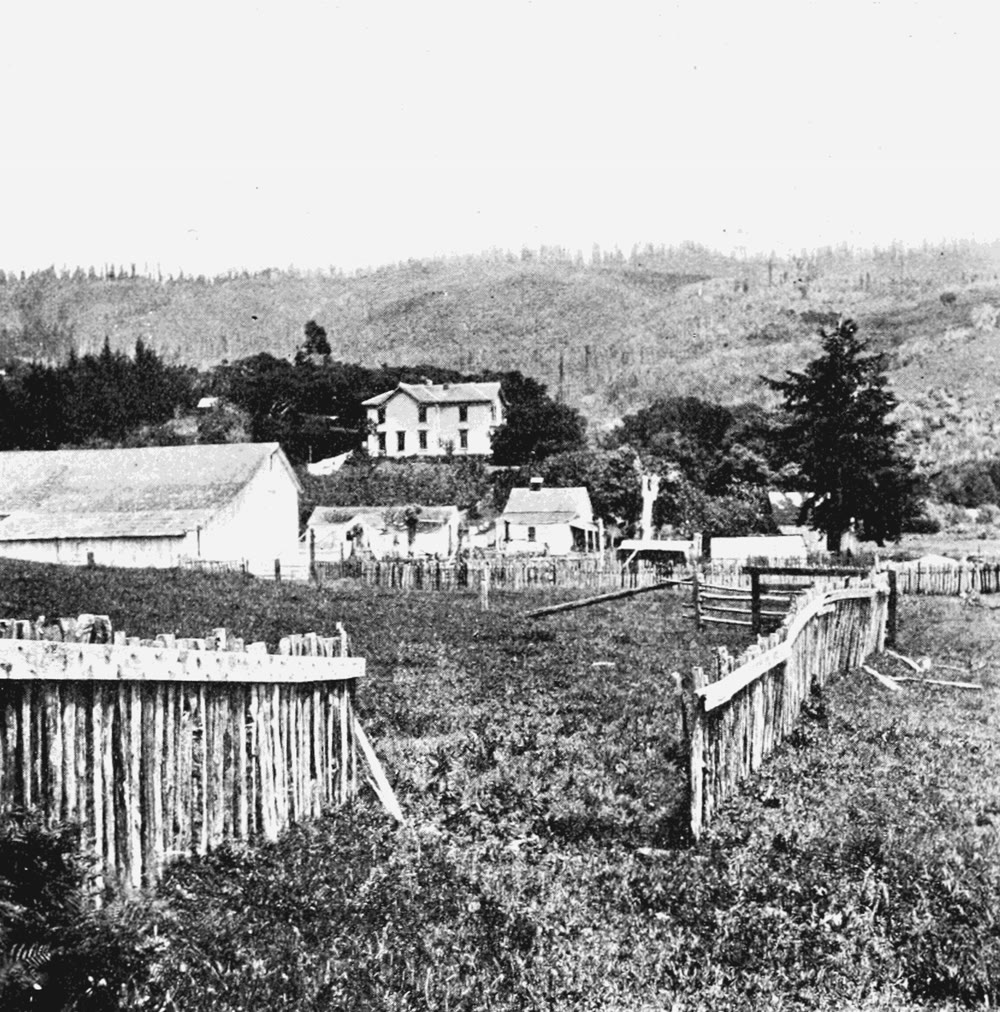
\includegraphics[height=5.6cm]{images/book3/b1-fence-1906.jpg}\hfill
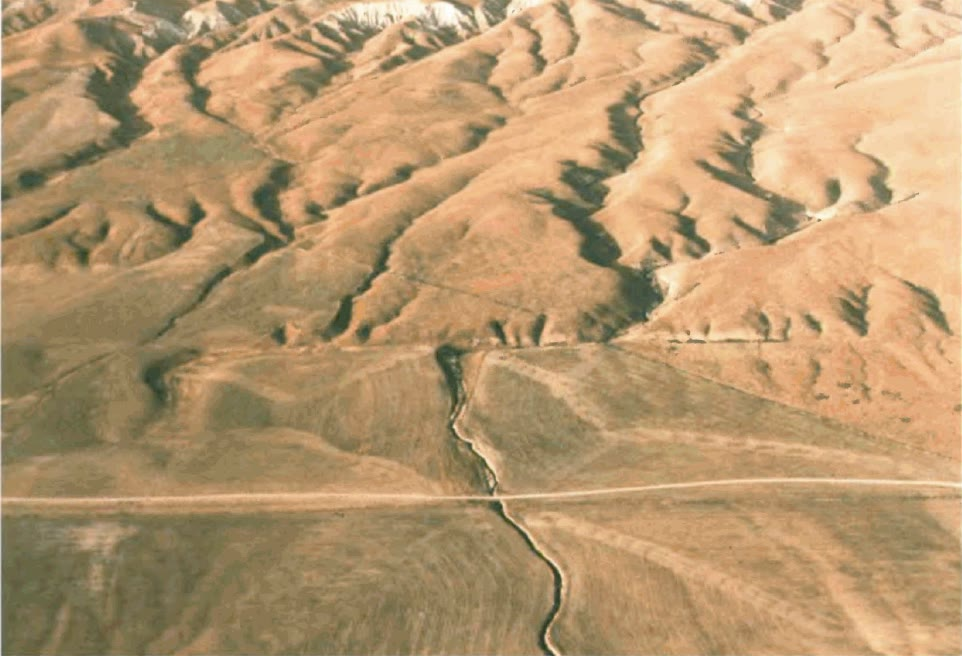
\includegraphics[height=5.6cm]{images/book3/b1-wallace-creek.jpg}
\par\smallskip{\small Links: hekken in landbouwgrond van Marin County, ten noorden van San Francisco, doorsneden door de breuk van 1906, gepubliceerd in datzelfde jaar onder de titel ``land separated by the earthquake fault''. Foto uit \emph{Popular Science Monthly}, vol.~69 (1906), publiek domein. Rechts: Wallace Creek, Carrizo Plain, van bovenaf gezien: de beek komt van de heuvels (boven), en waar zij de San Andreas-breuk kruist, aan de voet van de heuvels, springt haar bedding zijwaarts over \qty{130}{m}, de verschuiving die over duizenden jaren aardbevingen is opgebouwd. Foto: R.~E.~Wallace, U.S. Geological Survey, publiek domein. Beide van Wikimedia Commons.}
\label{fig:b1:earthquake-source:offsets}
\end{omfigure}
% ledger: commons:psm-fence, commons:wallace-creek

De uitspraak geeft een gemiddelde, geen dienstregeling. Bij Parkfield, op dezelfde breuk, werd een aardbeving van magnitude ongeveer 6 in 1857 gevolgd door vijf andere, heel gelijke, op hetzelfde traject van ongeveer \qty{30}{km}, met intervallen van bijna 22 jaar tot 1966; de volgende werd verwacht vóór 1993, en kwam in 2004, met een \omterm{def:b1:earthquake-source:mw}{momentmagnitude} van 6.0 en zonder duidelijk waarschuwingsteken. De sterkte van een breuk, de verschuiving van elke aardbeving en de belasting door haar buren variëren alle van de ene cyclus op de andere, en de \omterm{def:b1:earthquake-source:seismic-cycle}{seismische cyclus} wordt beter beschreven door een gemiddeld \omterm{def:b1:earthquake-source:seismic-cycle}{herhalingsinterval} en een spreiding eromheen dan door een periode.
% ledger: pp1515:parkfield, bl85:parkfield, usgs:hist-mw, bakun:2005

Sommige breuksegmenten vergrendelen helemaal niet. Tussen Parkfield en San Juan Bautista kruipt het centrale deel van de San Andreas-breuk: gestaag glijden op de breuk neemt bijna de hele beweging van de platen voor haar rekening, en er bouwt zich weinig of geen rek op aan weerszijden, zodat dit deel geen grote aardbevingen heeft; de grote breuk van 1857 begon aan haar zuidelijke einde, en die van 1906 stopte aan haar noordelijke. Een breuk die over een deel van haar oppervlak kruipt, is slechts ten dele vastgeklemd, en dat is de coëfficiënt $c$ van de propositie.
% ledger: pp1515:creep, pp1515:1906

\begin{inthefield}[Vorige aardbevingen lezen in een sleuf]
Instrumenten hebben aardbevingen pas iets meer dan een eeuw geregistreerd, veel minder dan één cyclus van de meeste breuken. Paleoseismologen verlengen het verslag door de grond te lezen. Een sleuf van enkele meters diep wordt gegraven dwars over een actieve breuk, waar lagen sediment ononderbroken zijn afgezet, in een moeras, een meer of een kleine alluviale waaier. Op haar wanden toont elke aardbeving zich als lagen die door de breuk zijn doorgesneden en verspringen en door jongere, ongebroken lagen worden bedekt; als een steilrand die door latere afzettingen is begraven; als zand dat vloeibaar werd en door scheuren omhoog kwam om over het oppervlak van die tijd uit te spreiden. Veen of plantenresten in de lagen net onder en net boven elke breuk worden met radiokoolstof gedateerd, en zo begrenzen zij de datum van elke aardbeving: één moeras op de San Andreas-breuk bewaart het verslag van twaalf. Langs kusten leggen vellen zand die door tsunami's zijn afgezet, en moerassen die plotseling een meter of zo zijn gezakt en onder getijdenmodder begraven zijn, de grote subductie-aardbevingen vast. Op de San Andreas-breuk kwam het meeste van de verschuiving in historische tijden met aardbevingen van magnitude 6 of meer.
\end{inthefield}
% ledger: pp1515:pallett, atwater:1987

\begin{history}[Harry Fielding Reid en de elastische terugveer]
Harry Fielding Reid, een Amerikaans natuurkundige, was lid van de staatscommissie die de aardbeving van 1906 bestudeerde. Door de posities te vergelijken van punten die in 1851--1865, in 1874--1892 en na de aardbeving waren opgemeten, vond hij dat verre punten aan de twee zijden van de San Andreas-breuk ten opzichte van elkaar ongeveer \qty{3.2}{m} waren verplaatst sinds de eerste meting, iets meer dan de helft van de verschuiving van ongeveer \qty{6}{m} op de breuk: een halve eeuw vóór de aardbeving was de rek die de breuk brak al half opgebouwd. Alleen elastische krachten konden de grond zo plotseling hebben verplaatst, en hij noemde de plotselinge terugkeer \omterm{def:b1:earthquake-source:seismic-cycle}{elastische terugveer}. Hij publiceerde het in het tweede deel van het verslag van de commissie, in 1910; het is nog steeds het voornaamste model van de aardbevingscyclus. Satellietpositionering heeft sindsdien de buiging gemeten die hij alleen had kunnen afleiden.
\end{history}
% ledger: reid:1910, pp1515:1906

\section{Seismisch moment en magnitude}\label{sec:b1:earthquake-source:moment}

De grootte van een aardbeving is de hoeveelheid verschuiving die zij maakte, over het oppervlak van de breuk dat glijdde, gewogen naar hoe stijf de gesteenten zijn.

\begin{definition}[Seismisch moment]\label{def:b1:earthquake-source:moment}
Laat een aardbeving met de gemiddelde hoeveelheid $D$ schuiven over een breuk van oppervlak $A$, in gesteenten met afschuifmodulus $\mu$ (de letter benoemt ook een wrijvingscoëfficiënt, in \cref{ch:b1:stress-strain-rheology}; de context maakt duidelijk welke). Haar \emph{seismisch moment}\index{seismisch moment} is
\[
  M_0 = \mu A D ,
\]
in newtonmeter.
\end{definition}
% ledger: usgs:gloss-moment

De eenheid is die van een koppel. Een verschuiving op een breuk zendt dezelfde golven uit als twee paar tegengestelde krachten, twee koppels, aangebracht in het hypocentrum, en het \omterm{def:b1:earthquake-source:moment}{seismisch moment} is het moment van elk koppel (deze gelijkwaardigheid, het dubbele koppel, wordt in Boek~5 bewezen). Het moment heeft de dimensie van een energie, maar het is er geen: de energie die als golven wordt uitgestraald, is er maar een klein deel van. Voor de gesteenten van de \omterm{def:b1:layered-earth:layers}{korst} wordt $\mu$ op \qty{30}{GPa} genomen.
% ledger: kanamori:1977, sk:mu-locking

De uitspraak wordt tegenwoordig berekend uit de langeperiodegolven die wereldwijd worden geregistreerd. Voor de aardbeving van Tohoku van 11 maart 2011 geeft de voorkeursoplossing van de U.S. Geological Survey $M_0 = \qty{5.59e22}{N.m}$. De breuk schoof over een oppervlak van ongeveer \qty{400}{km} lang en \qty{150}{km} breed; de definitie geeft dan de gemiddelde verschuiving
\[
  D = \frac{M_0}{\mu A}
    = \frac{\num{5.59e22}}{\num{3e10}\times\num{4e5}\times\num{1.5e5}}
    \approx \qty{31}{m} ,
\]
en modellen van de breuk vinden tot \qtyrange{50}{60}{m} in haar meest verplaatste deel.
% ledger: usgs:tohoku-mt, usgs:tohoku-summary

De magnitude uit Boek~1 is berekend uit de amplitude van de golven op een seismogram. Zulke magnitudes meten de golven van één periode; zodra een breuk veel langer is dan hun golflengte, enkele tot ongeveer vijftig kilometer, houdt de amplitude op met haar grootte te groeien, en de magnitude verzadigt. De magnitude van de lichaamsgolven verzadigt rond 6.5, die van de oppervlaktegolven rond 8.3. In 2011 was de eerste tsunamiwaarschuwing voor Tohoku gebaseerd op een magnitude van dit soort, die tekortschiet voor aardbevingen van magnitude 8 of meer, en de golven onderschatte. Het moment verzadigt niet, en de magnitude wordt nu eruit gedefinieerd.
% ledger: kanamori:1977, usgs:magtypes, jma:warning

\begin{definition}[Momentmagnitude]\label{def:b1:earthquake-source:mw}
De \emph{momentmagnitude}\index{momentmagnitude} van een aardbeving met \omterm{def:b1:earthquake-source:moment}{seismisch moment} $M_0$, in newtonmeter, is
\[
  M_w = \tfrac23\left(\log_{10} M_0 - 9.1\right) .
\]
\end{definition}
% ledger: usgs:magtypes

Thomas Hanks en Hiroo Kanamori definieerden de schaal in 1979, met de constante 9.05 in plaats van 9.1, een verschil van 0.03 in $M_w$; de constanten zijn gekozen om de oudere magnitudes te evenaren waar die niet verzadigen. De magnitude uit Boek~1 is, voor grote aardbevingen, dit getal: voor Tohoku
$M_w = \tfrac23(\log_{10}\num{5.59e22} - 9.1) = \tfrac23(22.75 - 9.1) = 9.1$;
de grote Chileense aardbeving van 1960 en de Alaska-aardbeving van 1964 hebben \omterm{def:b1:earthquake-source:mw}{momentmagnitudes} van 9.5 en 9.2, groottes die de oudere magnitudes niet konden tonen.
% ledger: hk:1979, kanamori:1977, usgs:hist-mw, usgs:tohoku-mt

\begin{proposition}[Eén eenheid magnitude]\label{prop:b1:earthquake-source:moment-steps}
Het \omterm{def:b1:earthquake-source:moment}{seismisch moment} is $M_0 = 10^{1.5 M_w + 9.1}$ newtonmeter. Eén eenheid \omterm{def:b1:earthquake-source:mw}{momentmagnitude} vermenigvuldigt het met $10^{1.5} \approx 31.6$, twee eenheden met $1000$. Als de uitgestraalde energie een vaste fractie van het moment is, groeit zij in dezelfde verhouding.
\end{proposition}

\begin{proof}
Het oplossen van de definitie voor $M_0$ geeft $\log_{10} M_0 = 1.5 M_w + 9.1$, en voor twee aardbevingen
\[
  \log_{10}\frac{M_0'}{M_0} = 1.5\,(M_w' - M_w) ,
\]
wat $1.5$ is voor één eenheid en $3$ voor twee. Als de uitgestraalde energie $E_s = k M_0$ is, met dezelfde $k$ voor beide, is $E_s'/E_s = M_0'/M_0$.
\end{proof}

Kanamori's benadering, $E_s \approx M_0/(2\times10^4)$ (aangenomen), is de veronderstelling van de laatste zin; de factor van ongeveer 32 in energie per eenheid magnitude, die in Boek~1 is ontmoet, is deze propositie. Aangezien $M_0 = \mu A D$ en de verschuiving van een aardbeving met de grootte van haar breuk groeit, heeft een grote magnitude een grote breuk nodig. De breuk van 1906, ongeveer \qty{430}{km} lang, brak de \omterm{def:b1:stress-strain-rheology:strength-envelope}{seismogene laag} tot ongeveer \qty{15}{km} met een gemiddelde verschuiving van enkele meters: met $D = \qty{4}{m}$, $M_0 = \num{3e10}\times\num{4.3e5}\times\num{1.5e4}
\times 4 = \qty{7.7e20}{N.m}$ en $M_w = 7.9$, de magnitude van de catalogus. Een magnitude van 9 vraagt een breuk van honderden kilometers lengte en meer dan honderd in breedte, wat alleen de flauw hellende grensvlakken van subductiezones bieden.
% ledger: kanamori:1977, pp1515:1906, usgs:hist-mw, usgs:pp1515-thatcher

\section{Focale mechanismen}\label{sec:b1:earthquake-source:focal}

De P-golf is de eerste die een seismometer bereikt. Haar \omterm{def:b1:earthquake-source:focal-mechanism}{eerste beweging}, de eerste uitslag van het verticale registratiesignaal, is omhoog waar de golf aankomt als een duw, waarbij de grond wordt samengedrukt en van de bron weg geworpen, en omlaag waar zij aankomt als een trek. Rond een aardbeving zijn duwen en trekken gerangschikt in een patroon dat de oriëntatie van de breuk en de richting van de verschuiving geeft.

\begin{proposition}[Het teken van de eerste beweging]\label{prop:b1:earthquake-source:first-motion}
Laat een breuk met opwaartse normaal $\mathbf n$ schuiven over de eenheidsvector $\mathbf d$ (de verschuiving van de \omterm{def:b1:faults-folds-fabrics:fault-elements}{hangende wand} ten opzichte van de \omterm{def:b1:faults-folds-fabrics:fault-elements}{liggende wand}). De P-golf die het hypocentrum verlaat in de eenheidsrichting $\mathbf x$, komt aan als een duw als $(\mathbf n\cdot\mathbf x)(\mathbf d\cdot\mathbf x) > 0$ en als een trek als $(\mathbf n\cdot\mathbf x)(\mathbf d\cdot\mathbf x) < 0$. De duwen en de trekken vullen zo vier kwadranten, gescheiden door het breukvlak ($\mathbf n\cdot\mathbf x = 0$) en door het vlak loodrecht op de verschuiving ($\mathbf d\cdot\mathbf x = 0$).
\end{proposition}

\begin{proof}
Een richting met $\mathbf n\cdot\mathbf x > 0$ wijst in de \omterm{def:b1:faults-folds-fabrics:fault-elements}{hangende wand}, die over $\mathbf d$ ten opzichte van de \omterm{def:b1:faults-folds-fabrics:fault-elements}{liggende wand} beweegt: het gesteente ervoor, waar $\mathbf d\cdot\mathbf x > 0$, wordt samengedrukt, en het gesteente erachter, waar $\mathbf d\cdot\mathbf x < 0$, wordt getrokken. Een richting met $\mathbf n\cdot\mathbf x < 0$ wijst in de \omterm{def:b1:faults-folds-fabrics:fault-elements}{liggende wand}, die over $-\mathbf d$ ten opzichte van de \omterm{def:b1:faults-folds-fabrics:fault-elements}{hangende wand} beweegt, dus zijn de tekens omgekeerd. In elk geval heeft de \omterm{def:b1:earthquake-source:focal-mechanism}{eerste beweging} het teken van $(\mathbf n\cdot\mathbf x)(\mathbf
d\cdot\mathbf x)$.
\end{proof}

Het argument geeft alleen het teken. De amplitude van de \omterm{def:b1:earthquake-source:focal-mechanism}{eerste beweging}, die evenredig is met $2(\mathbf n\cdot\mathbf x)(\mathbf d\cdot\mathbf x)$ en dus het grootst is onder \ang{45} van beide vlakken en nul erop, wordt hier aangenomen (Boek~5).

\begin{omfigure}
\begin{tikzpicture}[>={Stealth[length=5pt]}, font=\small, scale=0.95]
% map view around a vertical dextral fault striking north, the focus at the origin, rays leaving
% horizontally: pushes where (n.x)(d.x) > 0, i.e. in the NW and SE quadrants (beachballs.py,
% first_motion(0, 90, 180, x)). Stations at 20 azimuths on a circle of radius 2.3.
\fill[omThm!22] (0,0) -- (0,2.8) arc[start angle=90, end angle=180, radius=2.8] -- cycle;
\fill[omThm!22] (0,0) -- (0,-2.8) arc[start angle=270, end angle=360, radius=2.8] -- cycle;
\draw[black!40, line width=0.4pt] (0,0) circle[radius=2.8];
\draw[fault, line width=1.3pt] (0,-3.1) -- (0,3.1) node[above, font=\scriptsize] {breuk (knoopvlak)};
\draw[black, dashed, line width=0.7pt] (-3.1,0) -- (3.1,0) node[right, font=\scriptsize, align=left] {hulpvlak};
% slip: the west block moves north, the east block south
\draw[->, line width=1pt] (-0.3,-0.8) -- (-0.3,0.8);
\draw[->, line width=1pt] (0.3,0.8) -- (0.3,-0.8);
% stations
\foreach \a in {9,27,...,351} {
  \pgfmathsetmacro{\fm}{-sin(\a)*cos(\a)}  % (n.x)(d.x) with n = east, d = south, x = (sin a, cos a)
  \pgfmathparse{\fm>0 ? 1 : 0}
  \ifnum\pgfmathresult=1
    \fill[black] ({2.3*sin(\a)},{2.3*cos(\a)}) circle[radius=0.11];
  \else
    \draw[black, fill=white, line width=0.6pt] ({2.3*sin(\a)},{2.3*cos(\a)}) circle[radius=0.11];
  \fi
}
% P and T axes
\draw[<-, omProp, line width=1.1pt] ({0.7*sin(45)},{0.7*cos(45)}) -- ({1.6*sin(45)},{1.6*cos(45)}) node[above right, font=\scriptsize, inner sep=1pt] {P};
\draw[<-, omProp, line width=1.1pt] ({0.7*sin(225)},{0.7*cos(225)}) -- ({1.6*sin(225)},{1.6*cos(225)});
\draw[->, omProp, line width=1.1pt] ({0.7*sin(315)},{0.7*cos(315)}) -- ({1.6*sin(315)},{1.6*cos(315)}) node[above left, font=\scriptsize, inner sep=1pt] {T};
\draw[->, omProp, line width=1.1pt] ({0.7*sin(135)},{0.7*cos(135)}) -- ({1.6*sin(135)},{1.6*cos(135)});
\fill (0,0) circle[radius=0.06];
% legend
\begin{scope}[xshift=4.6cm, yshift=2.4cm]
  \fill[black] (0,0) circle[radius=0.11]; \node[anchor=west, font=\scriptsize] at (0.2,0) {duw: eerste beweging omhoog};
  \draw[black, fill=white, line width=0.6pt] (0,-0.5) circle[radius=0.11]; \node[anchor=west, font=\scriptsize] at (0.2,-0.5) {trek: eerste beweging omlaag};
  \fill[omThm!22] (-0.12,-1.12) rectangle (0.12,-0.88); \node[anchor=west, font=\scriptsize] at (0.2,-1.0) {compressiekwadrant};
  \draw[->] (-0.1,-1.6) -- (-0.1,-1.25); \node[anchor=west, font=\scriptsize] at (0.2,-1.42) {N};
\end{scope}
\end{tikzpicture}
\par\smallskip{\small \omterm{def:b1:earthquake-source:focal-mechanism}{Eerste bewegingen} rond een verticale rechtsdraaiende (dextrale) breuk die noord loopt, van bovenaf gezien, voor golven die het hypocentrum horizontaal verlaten naar stations rondom. Zwarte pijlen: de verschuiving van de twee blokken. De duwen vullen het noordwestelijke en het zuidoostelijke kwadrant, de trekken de andere twee; de breuk en het \omterm{def:b1:earthquake-source:focal-mechanism}{hulpvlak} scheiden ze. De \omterm{def:b1:earthquake-source:focal-mechanism}{P-as} (pijlen naar binnen) halveert de trekkwadranten, de \omterm{def:b1:earthquake-source:focal-mechanism}{T-as} (pijlen naar buiten) de duwkwadranten. Een sinistrale verschuiving op het gestreepte vlak, met het blok ten zuiden ervan dat naar het oosten beweegt, zou precies hetzelfde patroon geven (\cref{prop:b1:earthquake-source:auxiliary}).}
\label{fig:b1:earthquake-source:quadrants}
\end{omfigure}

Het product $(\mathbf n\cdot\mathbf x)(\mathbf d\cdot\mathbf x)$ verandert niet wanneer $\mathbf n$ en $\mathbf d$ worden verwisseld. Deze symmetrie is het centrale feit van de focale mechanismen.

\begin{definition}[Focaal mechanisme, knoopvlak, hulpvlak, P-as, T-as]\label{def:b1:earthquake-source:focal-mechanism}
De \emph{eerste beweging}\index{eerste beweging} van een P-golf bij een seismometer is de richting, omhoog of omlaag, van de eerste beweging van de grond op het verticale registratiesignaal. Het \emph{focaal mechanisme}\index{focaal mechanisme} van een aardbeving is de oriëntatie van het breukvlak en de richting van de verschuiving erop, zoals uit haar seismische golven gevonden. De twee loodrechte vlakken door het hypocentrum die de duwen van de trekken scheiden, zijn haar \emph{knoopvlakken}\index{knoopvlak}; één is het breukvlak, en het andere, loodrecht op de verschuiving, is het \emph{hulpvlak}\index{hulpvlak}. De \emph{P-as}\index{P-as} en de \emph{T-as}\index{T-as} zijn de richtingen op \ang{45} van beide knoopvlakken, in het midden van de trekkwadranten en van de duwkwadranten:
\[
  \mathbf P = \frac{\mathbf n - \mathbf d}{\sqrt2}, \qquad
  \mathbf T = \frac{\mathbf n + \mathbf d}{\sqrt2} .
\]
\end{definition}
% ledger: yvo:beachball, usgs:gloss-moment

\begin{proposition}[De twee knoopvlakken]\label{prop:b1:earthquake-source:auxiliary}
Een verschuiving $\mathbf d$ op het vlak met normaal $\mathbf n$ en een verschuiving $\mathbf n$ op het vlak met normaal $\mathbf d$ geven dezelfde \omterm{def:b1:earthquake-source:focal-mechanism}{eerste bewegingen} in elke richting. De \omterm{def:b1:earthquake-source:focal-mechanism}{eerste bewegingen} bepalen dus de twee \omterm{def:b1:earthquake-source:focal-mechanism}{knoopvlakken}, de P- en T-assen en de zin van de verschuiving op elk vlak, maar zij zeggen niet welk \omterm{def:b1:earthquake-source:focal-mechanism}{knoopvlak} de breuk is.
\end{proposition}

\begin{proof}
Het teken van $(\mathbf n\cdot\mathbf x)(\mathbf d\cdot\mathbf x)$ verandert niet door de verwisseling van $\mathbf n$ en $\mathbf d$; de vlakken $\mathbf n\cdot\mathbf x = 0$ en $\mathbf d\cdot\mathbf x = 0$ worden verwisseld, en $\mathbf n \pm \mathbf d$ blijft onveranderd. Een paar $(\mathbf n, \mathbf d)$ en het paar $(-\mathbf n, -\mathbf d)$, dat dezelfde verschuiving beschrijft gezien vanuit het andere blok, geven ook hetzelfde product. Niets in de \omterm{def:b1:earthquake-source:focal-mechanism}{eerste bewegingen} onderscheidt de twee beschrijvingen.
\end{proof}

Om te beslissen welk \omterm{def:b1:earthquake-source:focal-mechanism}{knoopvlak} heeft geschoven, gebruiken seismologen ander bewijs: het vlak waarlangs de naschokken op een rij liggen, de breuk aan het oppervlak, de plaatgrens waarop de aardbeving ligt. Voor de grote aardbeving van Sumatra--Andaman van 2004 helen de twee \omterm{def:b1:earthquake-source:focal-mechanism}{knoopvlakken} \ang{8} naar het noordoosten en \ang{83} naar het zuidwesten. De eerdere aardbevingen van de regio en de plaatmodellen plaatsen beide de zinkende plaat langs een vlak dat flauw naar het noordoosten helt, en het ondiepe vlak wordt als de breuk genomen: de aardbeving brak het plaatgrensvlak van de subductiezone, en haar naschokken verspreidden zich over meer dan \qty{1300}{km}.
% ledger: usgs:sumatra-mt, usgs:sumatra-summary

Omdat de \omterm{def:b1:earthquake-source:focal-mechanism}{P-as} in het midden van de trekken ligt en de \omterm{def:b1:earthquake-source:focal-mechanism}{T-as} in het midden van de duwen, worden zij vaak gelezen als de richtingen van de grootste en kleinste drukspanning, $\sigma_1$ en $\sigma_3$. Zij zijn er slechts benaderingen van. Een nieuwe breuk vormt zich onder $\ang{45} - \phi/2$ van $\sigma_1$, niet onder \ang{45} (\cref{ch:b1:stress-strain-rheology}), en een oude breuk kan onder nog een andere hoek glijden, zodat de assen van één aardbeving tientallen graden van de \omterm{def:b1:stress-strain-rheology:principal}{hoofdspanningen} kunnen liggen; de spanningen van een regio worden gevonden uit de mechanismen van vele aardbevingen samen.

Een \omterm{def:b1:earthquake-source:focal-mechanism}{focaal mechanisme} leeft op een bol rond het hypocentrum. Het wordt getekend op de onderste helft van die bol, die elke straal naar een verre station doorkruist, geprojecteerd op een schijf: een straal met eenheidsvector $\mathbf x = (E, N, U)$, met $U \le 0$, wordt uitgezet op
\[
  (X, Y) = \frac{(E, N)}{\sqrt{1 - U}} ,
\]
de verticale in het midden en de horizontale op de eenheidscirkel. Deze projectie behoudt oppervlakten (aangenomen; de projecties van de bol worden in Boek~5 bestudeerd), zodat elk kwadrant zijn juiste aandeel van de schijf bedekt. De duwkwadranten zijn gearceerd; het beeld heet een beachball.
% ledger: yvo:beachball

\begin{omfigure}
\begin{tikzpicture}[font=\small]
% lower-hemisphere equal-area beach balls, compressional quadrants shaded (figdata/bachelor-1/beachballs.py)
\foreach \n/\c/\t/\x in {normal/2/{(a) normaalbreuk\\ $090/60$, rake \ang{-90}}/0,
                         reverse/1/{(b) omgekeerde breuk\\ $090/30$, rake \ang{90}}/3.65,
                         strikeslip/2/{(c) strike-slip-breuk\\ $090/90$, rake \ang{180}}/7.3,
                         tohoku/2/{(d) Tohoku, 2011\\ $282/8$, rake \ang{78}}/10.95} {
  \begin{axis}[at={(\x cm,0)}, anchor=center, width=2.9cm, height=2.9cm, scale only axis,
      axis equal image, xmin=-1.04, xmax=1.04, ymin=-1.04, ymax=1.04, hide axis, clip=false]
    \fill[white] (axis cs:0,0) circle[radius=1];
    \addplot[fill=omThm!55, draw=none] table[x=X, y=Y] {figdata/out/bachelor-1-beachballs-\n-c1.dat};
    \ifnum\c=2
      \addplot[fill=omThm!55, draw=none] table[x=X, y=Y] {figdata/out/bachelor-1-beachballs-\n-c2.dat};
    \fi
    \addplot[black, line width=0.6pt] table[x=X, y=Y] {figdata/out/bachelor-1-beachballs-\n-p1.dat};
    \addplot[black, line width=0.6pt] table[x=X, y=Y] {figdata/out/bachelor-1-beachballs-\n-p2.dat};
    \draw[black, line width=0.8pt] (axis cs:0,0) circle[radius=1];
    \draw[black, line width=0.5pt] (axis cs:0,1) -- (axis cs:0,1.12) node[above, font=\scriptsize, inner sep=1pt] {N};
    \addplot[only marks, mark=none, nodes near coords={\textbf{P}}, nodes near coords align=center, every node near coord/.append style={font=\scriptsize, inner sep=0pt}] table[x=X, y=Y] {figdata/out/bachelor-1-beachballs-\n-P.dat};
    \addplot[only marks, mark=none, nodes near coords={\textbf{T}}, nodes near coords align=center, every node near coord/.append style={font=\scriptsize, inner sep=0pt}] table[x=X, y=Y] {figdata/out/bachelor-1-beachballs-\n-T.dat};
    \node[anchor=north, align=center, font=\scriptsize] at (axis cs:0,-1.12) {\t};
  \end{axis}
}
\end{tikzpicture}
\par\smallskip{\small Beachballs: het onderste halfrond rond het hypocentrum in gelijke-oppervlakteprojectie, noord boven, de duwkwadranten gearceerd, en P en T die de assen aangeven (een letter wordt naar binnen verplaatst wanneer haar as nabij de rand ligt). Elk mechanisme is gegeven door de ligging van één \omterm{def:b1:earthquake-source:focal-mechanism}{knoopvlak}, richtingshelling en helling, en de \omterm{def:b1:faults-folds-fabrics:fault-elements}{rake} van de verschuiving erop. (a) Een \omterm{def:b1:faults-folds-fabrics:fault-types}{normaalbreuk} die \ang{60} oostwaarts helt: het trekkwadrant vult het midden. (b) Een \omterm{def:b1:faults-folds-fabrics:fault-types}{omgekeerde breuk} die \ang{30} oostwaarts helt: het duwkwadrant vult het midden. (c) Een verticale \omterm{def:b1:faults-folds-fabrics:fault-types}{strike-slip-breuk}: vier kwadranten die in het midden samenkomen. (d) De aardbeving van Tohoku van 2011 (momenttensor van de U.S. Geological Survey): een \omterm{def:b1:faults-folds-fabrics:fault-types}{overschuiving} op een vlak dat \ang{8} naar $282$ helt, onder Japan, met het steile \omterm{def:b1:earthquake-source:focal-mechanism}{hulpvlak} in het oosten.}
\label{fig:b1:earthquake-source:beachballs}
\end{omfigure}
% ledger: usgs:tohoku-mt

Seismologen geven een mechanisme door de \omterm{def:b1:geological-maps:attitude}{strijk}, helling en \omterm{def:b1:faults-folds-fabrics:fault-elements}{rake} van elk \omterm{def:b1:earthquake-source:focal-mechanism}{knoopvlak}; de \omterm{def:b1:geological-maps:attitude}{strijk} is de richting van de helling min \ang{90}, zoals in \cref{ch:b1:faults-folds-fabrics}. Voor Tohoku zijn de vlakken $192/8/78$ en $24/81/91$ in \omterm{def:b1:geological-maps:attitude}{strijk}, helling en \omterm{def:b1:faults-folds-fabrics:fault-elements}{rake}, en de P- en T-assen lopen naar $113$ en $296$ en hun \omterm{def:b1:field-lab-methods-1:trend-plunge}{duik} is \ang{36} en \ang{53}. Het \omterm{def:b1:earthquake-source:focal-mechanism}{hulpvlak} volgt uit het breukvlak: zijn normaal is $\mathbf d$ en zijn verschuiving is $\mathbf n$, dus wordt het gevonden door $\mathbf n$ en $\mathbf d$ uit de \omterm{def:b1:geological-maps:attitude}{strijk}, helling en \omterm{def:b1:faults-folds-fabrics:fault-elements}{rake} te berekenen, ze te verwisselen, en de \omterm{def:b1:geological-maps:attitude}{strijk}, helling en \omterm{def:b1:faults-folds-fabrics:fault-elements}{rake} terug af te lezen (oefening~\ref{exo:b1:earthquake-source:7}).
% ledger: usgs:tohoku-mt

\begin{method}[Een beachball lezen]\label{met:b1:earthquake-source:beachball}
\begin{enumerate}
  \item Kijk naar het midden, dat de verticale is. Gearceerd (een duw recht naar beneden): een omgekeerde of overschuivingscomponent; wit: een normale component. Twee rechte diameters die in het midden kruisen: een strike-slip-mechanisme.
  \item Zoek de twee \omterm{def:b1:earthquake-source:focal-mechanism}{knoopvlakken}, de krommen die de kwadranten begrenzen. Een vlak door het midden is verticaal; een vlak helt naar de kant van het midden waarop zijn kromme ligt, des te flauwer naarmate de kromme dichter bij de rand ligt.
  \item Zoek de \omterm{def:b1:earthquake-source:focal-mechanism}{T-as} in het midden van de gearceerde kwadranten en de \omterm{def:b1:earthquake-source:focal-mechanism}{P-as} in het midden van de witte: de grond werd langs P verkort en langs T verlengd.
  \item Lees of bereken voor elk \omterm{def:b1:earthquake-source:focal-mechanism}{knoopvlak} de \omterm{def:b1:faults-folds-fabrics:fault-elements}{rake}, en benoem de breuk die het zou zijn met \cref{def:b1:faults-folds-fabrics:fault-types}. De twee vlakken delen altijd de dip-slip-zin, normaal of omgekeerd, en hebben tegengestelde strike-slip-zinnen: een strike-slip-mechanisme geeft één \omterm{def:b1:faults-folds-fabrics:fault-types}{dextraal} en één \omterm{def:b1:faults-folds-fabrics:fault-types}{sinistraal} vlak.
  \item Kies het breukvlak uit de naschokken, de geologie of de plaatgrens.
\end{enumerate}
\end{method}

\begin{inthelab}[Op een seismologisch observatorium]
\begin{minipage}[t]{0.6\linewidth}\vspace{0pt}
Binnen enkele minuten na een grote aardbeving zijn haar golven door honderden stations geregistreerd, en de gegevens bereiken de analisten van de observatoria bijna in reële tijd. De eerste aankomsten van de P-golf, die later bij de stations aankomen naarmate zij verder weg zijn, worden op de registraties afgelezen om het hypocentrum te plaatsen. Daarna worden de lange, trage golven die in de volgende tientallen minuten worden geregistreerd, vergeleken met golven die voor proefbronnen zijn berekend; de bron waarvan de golven het best passen, geeft de momenttensor, die tegelijk het \omterm{def:b1:earthquake-source:moment}{seismisch moment}, de \omterm{def:b1:earthquake-source:mw}{momentmagnitude} en de twee \omterm{def:b1:earthquake-source:focal-mechanism}{knoopvlakken} bevat. Voor kleine aardbevingen, te zwak daarvoor, lezen de analisten de \omterm{def:b1:earthquake-source:focal-mechanism}{eerste bewegingen} op de dichtstbijzijnde registraties af en passen de \omterm{def:b1:earthquake-source:focal-mechanism}{knoopvlakken} erop aan
op de manier die in deze paragraaf is beschreven. Elke oplossing wordt met haar onzekerheden gepubliceerd en herzien naarmate er meer gegevens binnenkomen.
\end{minipage}\hfill
\begin{minipage}[t]{0.36\linewidth}\vspace{0pt}
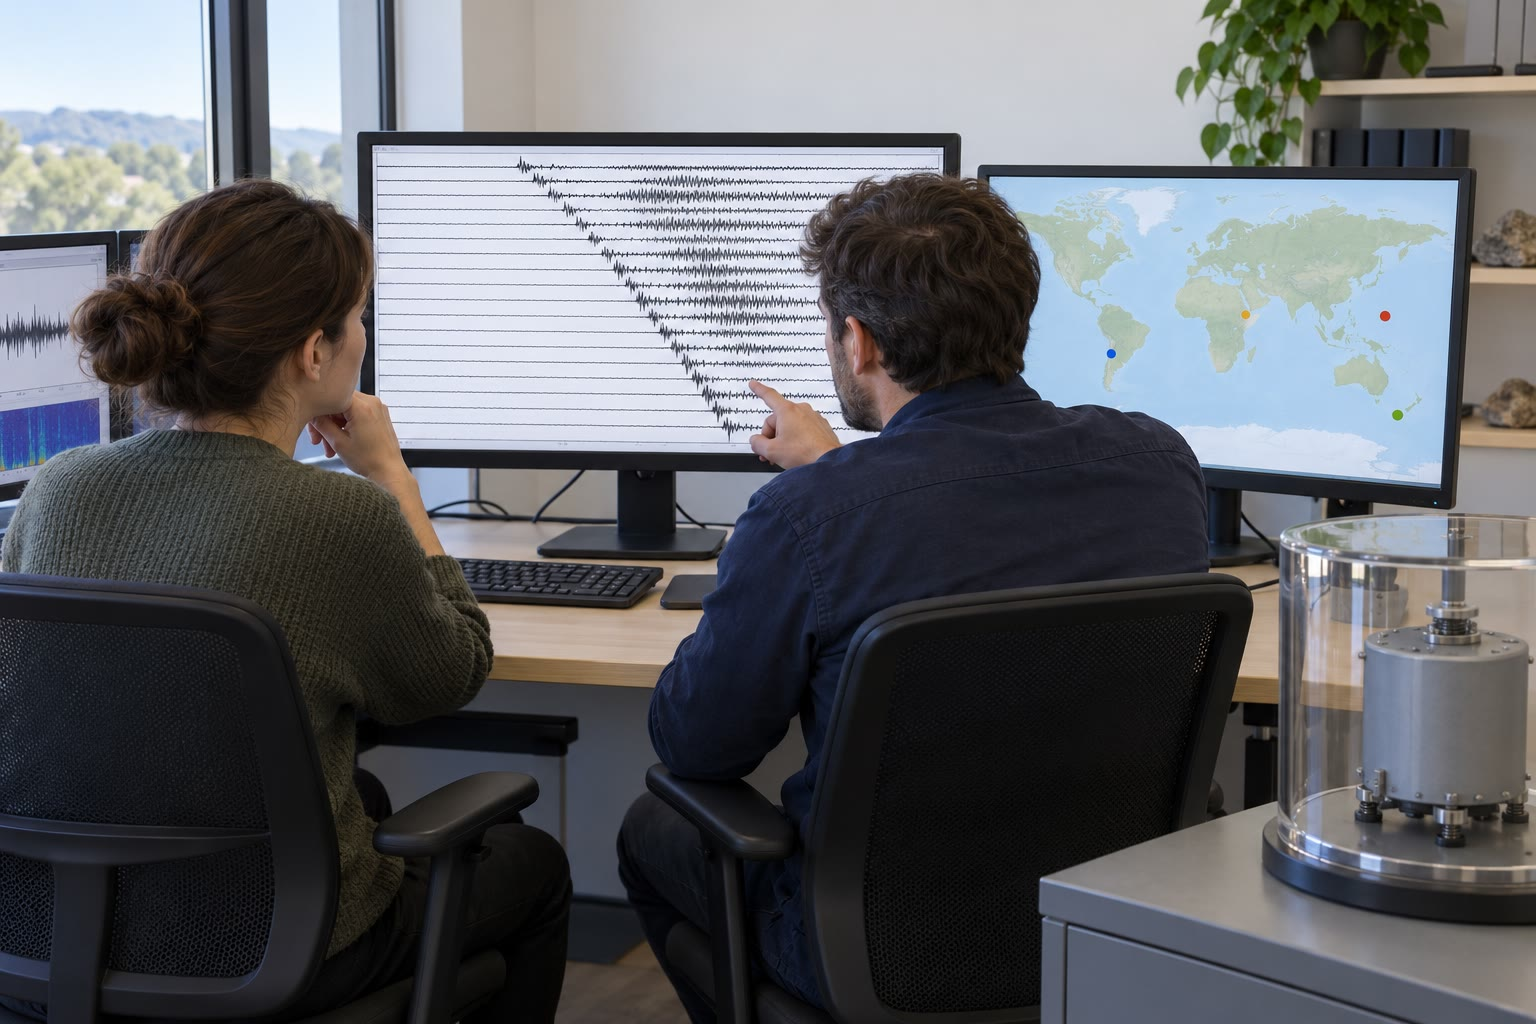
\includegraphics[width=\linewidth]{images/book3/ai/b1-seismic-analysis.jpg}

{\scriptsize Seismologen lezen een registratiesectie, de sporen van één aardbeving bij stations gesorteerd naar afstand (AI-illustratie).}
\end{minipage}
\end{inthelab}
% ledger: yvo:beachball

\section{De belasting meten: geodesie}\label{sec:b1:earthquake-source:geodesy}

Tussen aardbevingen is een vastgeklemde breuk onzichtbaar voor seismometers, maar de grond eromheen beweegt. Permanente satellietpositioneringsstations meten die beweging, en de manier waarop hun snelheden over een breuk veranderen, vertelt hoe diep zij is vastgeklemd.

\begin{definition}[Vastklemdiepte]\label{def:b1:earthquake-source:locking-depth}
De \emph{vastklemdiepte}\index{vastklemdiepte} van een breuk is de diepte waartoe zij tussen aardbevingen is vastgeklemd, de breuk daaronder glijdt gestaag met de langetermijnsnelheid; het is de diepte van het deel van de breuk dat in de volgende aardbeving schuift.
\end{definition}
% ledger: usgs:pp1515-thatcher

\begin{proposition}[Interseismische snelheid over een strike-slip-breuk]\label{prop:b1:earthquake-source:interseismic}
Laat een verticale \omterm{def:b1:faults-folds-fabrics:fault-types}{strike-slip-breuk} in een elastische halfruimte van het oppervlak tot de diepte $D$ vastgeklemd zijn, en onder die diepte met de snelheid $V$ schuiven. De snelheid van het oppervlak evenwijdig aan de breuk, op de afstand $x$ ervan, is
\[
  v(x) = \frac{V}{\pi}\arctan\frac{x}{D} .
\]
Als de breuk dan met $s$ van het oppervlak tot de diepte $D$ schuift in een aardbeving, verplaatst het oppervlak zich over $u(x) = (s/\pi)\arctan(D/x)$ voor $x > 0$, en over $-u(-x)$ voor $x < 0$.
\end{proposition}
\admitted

Dit model, van Savage en Burford, is de eenvoudigste vorm van de \omterm{def:b1:earthquake-source:seismic-cycle}{elastische terugveer}, en de kromme van het hek van de eerste figuur. Haar eigenschappen volgen uit de formule.

\begin{proposition}[Het interseismische profiel lezen]\label{prop:b1:earthquake-source:profile}
In het model van \cref{prop:b1:earthquake-source:interseismic}:
\begin{enumerate}[label=(\alph*)]
  \item ver van de breuk neigt de snelheid naar $\pm V/2$, waarbij de twee platen met $V$ ten opzichte van elkaar bewegen;
  \item de helft van de verandering van snelheid over de breuk gebeurt binnen de afstand $D$ ervan: $v(\pm D) = \pm V/4$;
  \item de snelheid van de \omterm{def:b1:stress-strain-rheology:strain}{schuifrek} van het oppervlak, $\mathrm dv/\mathrm dx$, is het grootst op de breuk, waar zij gelijk is aan $V/(\pi D)$;
  \item als de breuk, na belasting gedurende de tijd $t$, met $s = Vt$ schuift in een aardbeving, eindigt de grond overal aan weerszijden verplaatst over $\pm s/2$: de cyclus laat geen permanente buiging achter, alleen de verspringing $s$ op de breuk.
\end{enumerate}
\end{proposition}

\begin{proof}
(a) $\arctan(x/D) \to \pm\pi/2$ als $x \to \pm\infty$. (b) $\arctan 1 = \pi/4$, dus $v(D) = V/4$, en $v$ is oneven. (c) $\mathrm dv/\mathrm dx = (V/\pi D)/(1 +
x^2/D^2)$, het grootst bij $x = 0$. (d) Voor $x > 0$ heeft de belasting de grond verplaatst met $t\,v(x) = (s/\pi)\arctan(x/D)$ en de aardbeving met
$(s/\pi)\arctan(D/x)$; omdat $\arctan y + \arctan(1/y) = \pi/2$ voor $y > 0$ is de som $s/2$. Hetzelfde geldt met de tekens omgekeerd voor $x < 0$.
\end{proof}

Eigenschap (b) geeft de \omterm{def:b1:earthquake-source:locking-depth}{vastklemdiepte} uit een profiel van stations: het is de afstand tot de breuk waarop de snelheid met een kwart van $V$ is veranderd ten opzichte van haar waarde op de breuk. Een ondiepe vergrendeling concentreert de rek nabij de breuk (de figuur hieronder), een diepe spreidt haar over een brede gordel.
Langs het systeem van de San Andreas-breuk lopen de \omterm{def:b1:earthquake-source:locking-depth}{vastklemdiepten} uit de geodesie van bijna 0, op kruipende segmenten, tot \qty{26}{km}, en komen zij overeen met de diepten van de aardbevingen: het vastgeklemde deel is de \omterm{def:b1:stress-strain-rheology:strength-envelope}{seismogene laag} van \cref{ch:b1:stress-strain-rheology}. Voor een verschuivingssnelheid van \qty{34}{mm.yr^{-1}} en een \omterm{def:b1:earthquake-source:locking-depth}{vastklemdiepte} van \qty{15}{km} is de schuifreksnelheid op de breuk $\num{0.034}/(\pi\times\num{15000}) = \num{7.2e-7}$ per jaar, wat een lijn over de breuk minder dan een millimeter per kilometer per jaar buigt, en toch over twee eeuwen de enkele meters verschuiving van een grote aardbeving opslaat.
% ledger: sk:mu-locking, usgs:pp1515-wallace, usgs:pp1515-thatcher

\begin{omfigure}
\begin{tikzpicture}[font=\small]
\begin{axis}[omrecord, width=11cm, height=5.6cm, xmin=-100, xmax=100, ymin=-19, ymax=19,
    xlabel={afstand tot de breuk $x$ (km)}, ylabel={snelheid $v$ (\unit{mm.yr^{-1}})},
    legend style={font=\scriptsize, at={(0.02,0.96)}, anchor=north west}, legend cell align=left]
  \addplot[omDef, line width=0.9pt, dashed] table[x=x, y=v5] {figdata/out/bachelor-1-interseismic-profiles.dat};
  \addplot[omThm, line width=1.1pt] table[x=x, y=v15] {figdata/out/bachelor-1-interseismic-profiles.dat};
  \addplot[omProp, line width=0.9pt, dotted] table[x=x, y=v25] {figdata/out/bachelor-1-interseismic-profiles.dat};
  \legend{$D = \qty{5}{km}$, $D = \qty{15}{km}$, $D = \qty{25}{km}$}
  \draw[black!50, dashed] (axis cs:-100,17) -- (axis cs:100,17);
  \draw[black!50, dashed] (axis cs:-100,-17) -- (axis cs:100,-17);
  \node[anchor=north west, font=\scriptsize] at (axis cs:-30,17) {$+V/2$};
  \node[anchor=south west, font=\scriptsize] at (axis cs:30,-17) {$-V/2$};
  \draw[black!60] (axis cs:0,-19) -- (axis cs:0,19);
  \node[anchor=east, font=\scriptsize] at (axis cs:-1,5) {breuk};
\end{axis}
\end{tikzpicture}
\par\smallskip{\small Snelheid van de grond evenwijdig aan een vastgeklemde \omterm{def:b1:faults-folds-fabrics:fault-types}{strike-slip-breuk}, ten opzichte van het spoor van de breuk, voor een verschuivingssnelheid $V = \qty{34}{mm.yr^{-1}}$, die van de San Andreas-breuk bij Wallace Creek, en drie \omterm{def:b1:earthquake-source:locking-depth}{vastklemdiepten} (\cref{prop:b1:earthquake-source:interseismic}). Hoe ondieper de vergrendeling, hoe smaller de gordel waarin de snelheid verandert.}
\label{fig:b1:earthquake-source:interseismic}
\end{omfigure}
% ledger: usgs:pp1515-wallace

Satellietpositionering meet de grond op een paar stations. Radarsatellieten meten haar overal: twee radarbeelden van hetzelfde gebied, vanuit dezelfde baan op verschillende tijdstippen genomen, worden golf voor golf vergeleken, en het verschil van fase brengt de verandering van de afstand tussen de grond en de satelliet in kaart, punt voor punt, honderd meter uit elkaar, zonder dat vooraf een netwerk van stations is opgesteld. De eerste zulke kaart, van een grote Californische aardbeving in 1992, toonde haar verplaatsing tijdens de aardbeving in één beeld en kwam overeen met de verschuiving die op het veld en door landmeting was gemeten; de techniek, radarinterferometrie, hoort bij Boek~5.
% ledger: massonnet:1993

\section{Hoe vaak: de wet van Gutenberg--Richter}\label{sec:b1:earthquake-source:gr}

Kleine aardbevingen komen veel vaker voor dan grote, en op een opmerkelijk regelmatige manier.

\begin{proposition}[Wet van Gutenberg--Richter]\label{prop:b1:earthquake-source:gutenberg-richter}
In een regio en een periode\index{wet van Gutenberg--Richter}, volgt het aantal $N$ aardbevingen van magnitude ten minste
$M$ de volgende wet:
\[
  \log_{10} N = a - bM ,
\]
voor elke $M$ boven de \omterm{def:b1:earthquake-source:b-value}{magnitude van volledigheid} van de catalogus, met constanten $a$ en $b$ die van de regio afhangen; $b$ ligt in de meeste actieve regio's dicht bij 1.
\end{proposition}
\admitted
% ledger: fd:1993, gr:1944

De wet is het resultaat van waarneming, gepubliceerd door Beno Gutenberg en Charles Richter voor Californië in 1944 en sindsdien overal teruggevonden; nog geen theorie leidt haar af, noch de waarde van $b$.
% ledger: gr:1944

\begin{definition}[b-waarde, magnitude van volledigheid]\label{def:b1:earthquake-source:b-value}
De constante $b$ van de \omterm{prop:b1:earthquake-source:gutenberg-richter}{wet van Gutenberg--Richter} van een regio is haar \emph{b-waarde}\index{b-waarde}. De \emph{magnitude van volledigheid}\index{magnitude van volledigheid} van een catalogus is de kleinste magnitude waarboven zij elke aardbeving van de regio en de periode registreert.
\end{definition}

Een \omterm{def:b1:earthquake-source:b-value}{b-waarde} van 1 betekent voor elke eenheid magnitude erbij tien keer minder aardbevingen.
Onder de \omterm{def:b1:earthquake-source:b-value}{magnitude van volledigheid} blijven de aantallen achter bij de lijn, omdat kleine aardbevingen door te weinig stations worden geregistreerd om te worden gelokaliseerd: de wet lijkt te buigen, en $b$ moet erboven worden gemeten. Voor de hele Aarde, verdeeld in ondiepe, tussenliggende en diepe aardbevingen, liggen de gemeten waarden tussen 0.72 en 1.34, maar zij verschillen met \qty{30}{\percent} of meer van de ene catalogus, het ene magnitudebereik of de andere methode tot de andere: een waarde ver van 1 is in de eerste plaats een reden om de catalogus na te gaan.
% ledger: fd:1993

\begin{omfigure}
\begin{tikzpicture}[font=\small]
\begin{axis}[omrecord, width=6.4cm, height=5.8cm, ymode=log, xmin=5.8, xmax=9.3, ymin=0.01, ymax=300,
    xlabel={magnitude $M$}, ylabel={aardbevingen van magnitude $\ge M$ per jaar},
    log basis y=10, title={(a) frequentie en magnitude}, title style={font=\small}]
  \addplot[omProp, line width=0.9pt, domain=5.8:9.3] table[x=M, y=rate] {figdata/out/bachelor-1-gutenberg_richter-fit.dat};
  \addplot[only marks, mark=*, mark size=1.3pt, omDef] table[x=M, y=rate] {figdata/out/bachelor-1-gutenberg_richter-counts.dat};
  \draw[black!50, dashed] (axis cs:7.5,0.01) -- (axis cs:7.5,300);
  \node[anchor=south west, font=\scriptsize, omProp] at (axis cs:8.45,0.5) {$b = 1.01$};
  \node[anchor=north west, font=\scriptsize, align=left] at (axis cs:7.55,200) {gefit over\\ $6.0 \le M \le 7.5$};
\end{axis}
\begin{axis}[omrecord, at={(7.6cm,0)}, width=6.4cm, height=5.8cm, xmin=5.8, xmax=9.3, ymin=0, ymax=1.05,
    xlabel={magnitude $M$}, ylabel={aandeel van het moment van aardbevingen $\ge M$},
    title={(b) waar het moment naartoe gaat}, title style={font=\small}]
  \addplot[const plot, omDef, line width=0.9pt] table[x=M, y=share] {figdata/out/bachelor-1-gutenberg_richter-moment.dat};
\end{axis}
\end{tikzpicture}
\par\smallskip{\small De \num{7031} aardbevingen van magnitude 6 of meer in de wereld, 1976--2025 (catalogus van de U.S. Geological Survey). (a) Het jaarlijkse aantal aardbevingen van magnitude ten minste $M$; de lijn is de kleinste-kwadratenfit van $\log_{10} N$ tegen $M$ van 6.0 tot 7.5, waar elk aantal boven 200 ligt: $\log_{10} N = 8.20 - 1.01\,M$ per jaar. Boven magnitude 8 vallen de weinige gebeurtenissen onder de lijn. (b) Het aandeel van het totale seismische moment dat wordt vrijgegeven door de aardbevingen van magnitude ten minste $M$, elk moment berekend als $10^{1.5M + 9.1}$\,\unit{N.m}: de 40 aardbevingen van magnitude 8 of meer gaven \qty{63}{\percent} ervan vrij.}
\label{fig:b1:earthquake-source:gutenberg-richter}
\end{omfigure}
% ledger: data:usgs-comcat (fit and shares computed in figdata/bachelor-1/gutenberg_richter.py)

Voor de wereldcatalogus van de figuur voorspelt de wet met $a = 8.20$ en $b = 1.01$ 14 aardbevingen van magnitude 7 of meer per jaar, zoals waargenomen, en 1.35 van magnitude 8 of meer, terwijl er 40 in vijftig jaar, 0.8 per jaar, werden geregistreerd. Of de grootste aardbevingen werkelijk minder zijn dan de lijn, zoals de eindige grootte van breuken zou suggereren, of alleen zo zeldzaam dat zij in vijftig jaar ontbreken, wordt door zo weinig gebeurtenissen niet beslist. Ongeveer één op de negen magnitudes in deze catalogus is een oppervlaktegolf- of lichaamsgolfmagnitude, die verzadigen; de grootste gebeurtenissen hebben allemaal \omterm{def:b1:earthquake-source:mw}{momentmagnitudes}.
% ledger: data:usgs-comcat

De vele kleine aardbevingen doen weinig van het werk. Hun aantal groeit tien keer voor elke eenheid magnitude minder, maar hun momenten worden 31.6 keer kleiner.

\begin{proposition}[De grootste aardbevingen geven het meeste moment vrij]\label{prop:b1:earthquake-source:largest}
Laat aardbevingen de \omterm{prop:b1:earthquake-source:gutenberg-richter}{wet van Gutenberg--Richter} volgen met $b < 1.5$, tot een grootste magnitude $M_{\max}$, en laat zij worden gegroepeerd in klassen van één eenheid magnitude breed, de bovenste klasse eindigend bij $M_{\max}$. Dan geven de aardbevingen van de bovenste klasse meer dan de fractie $1 - 10^{-(1.5 - b)}$ van het totale moment vrij, hoe klein ook de kleinste geteldde magnitude is: meer dan \qty{68}{\percent} voor $b = 1$.
\end{proposition}

\begin{proof}
Laat de klassen genummerd zijn $k = 0, 1, \dots, K$ vanaf de kleinste, de klasse $k$ loopt van $M_k$ tot $M_k + 1$, met $M_{k+1} = M_k + 1$. Volgens de wet is het aantal aardbevingen in klasse $k$ $10^{a - bM_k} - 10^{a - b(M_k+1)} =
10^{a - bM_k}(1 - 10^{-b})$; volgens \cref{prop:b1:earthquake-source:moment-steps}
ligt het moment van elk tussen $10^{1.5M_k + 9.1}$ en $10^{1.5}$ keer dat, en omdat elke klasse de vorige is verschoven over één eenheid, is het moment van
klasse $k$ gelijk aan $C q^k$ voor een constante $C$ en de verhouding
$q = 10^{-b}\times10^{1.5} = 10^{1.5 - b} > 1$. Het totaal is de meetkundige som
\[
  S = C(1 + q + \dots + q^K) = C\,\frac{q^{K+1} - 1}{q - 1} ,
\]
en het aandeel van de bovenste klasse is
\[
  \frac{C q^K}{S} = \frac{q^K (q - 1)}{q^{K+1} - 1}
  > \frac{q^K (q - 1)}{q^{K+1}} = 1 - \frac1q = 1 - 10^{-(1.5 - b)} .
\]
Voor $b = 1$ is $1 - 10^{-0.5} = 0.684$.
\end{proof}

In de wereldcatalogus is het aandeel van deze orde: de bovenste eenheid van magnitude, van 8.1 tot 9.1, gaf meer dan de helft van het moment van vijftig jaar vrij, en de twee grootste aardbevingen, Sumatra--Andaman in 2004 en Tohoku in 2011, met magnitudes van 9.1, gaven er \qty{29}{\percent} van op zichzelf vrij. Het moment dat een plaatgrens moet vrijgeven, wordt bepaald door haar verschuivingssnelheid; de propositie zegt dat het bijna geheel in haar grootste aardbevingen wordt vrijgegeven, en dat de vele kleine, hoe frequent ook, een breuk niet ontlasten van de volgende grote.
% ledger: data:usgs-comcat, usgs:sumatra-mt, usgs:tohoku-mt

\section{Oefeningen}

\begin{exercise}[$\star$]\label{exo:b1:earthquake-source:1}
(a) Bereken de \omterm{def:b1:earthquake-source:mw}{momentmagnitude} van een aardbeving met een \omterm{def:b1:earthquake-source:moment}{seismisch moment} van \qty{4e17}{N.m}. (b) De aardbeving van Tohoku had $M_0 = \qty{5.59e22}{N.m}$: controleer haar magnitude. (c) Welk \omterm{def:b1:earthquake-source:moment}{seismisch moment} heeft een aardbeving van magnitude 7.0?
% ledger: usgs:tohoku-mt
\end{exercise}

\begin{exercise}[$\star$]\label{exo:b1:earthquake-source:2}
Een \omterm{def:b1:faults-folds-fabrics:fault-types}{strike-slip-breuk} wordt belast met \qty{25}{mm.yr^{-1}}, en haar aardbevingen schuiven elk ongeveer \qty{3}{m}. (a) Wat is hun \omterm{def:b1:earthquake-source:seismic-cycle}{herhalingsinterval} als de breuk er tussen hen volledig vastzit? (b) En als de helft van de verschuivingssnelheid door gestaag kruipen wordt opgenomen?
\end{exercise}

\begin{exercise}[$\star$]\label{exo:b1:earthquake-source:3}
Bepaal hoeveel keer groter het \omterm{def:b1:earthquake-source:moment}{seismisch moment} van een aardbeving van magnitude 7.4 is dan dat van een aardbeving van magnitude 6.2, en hoeveel aardbevingen van magnitude 6.2 hetzelfde moment zouden vrijgeven.
\end{exercise}

\begin{exercise}[$\star$]\label{exo:b1:earthquake-source:4}
In een regio met $b = 1$ worden elk jaar duizend aardbevingen van magnitude 3 of meer geregistreerd. Bereken hoeveel van magnitude 5 of meer en van magnitude 6 of meer elk jaar worden verwacht. Bepaal de gemiddelde tijd tussen aardbevingen van magnitude 7 of meer.
\end{exercise}

\begin{exercise}[$\star\star$]\label{exo:b1:earthquake-source:5}
De aardbeving van 1906 brak de San Andreas-breuk over ongeveer \qty{430}{km}. (a) Neem aan dat de breuk tot \qty{15}{km} diep reikte met een gemiddelde verschuiving van \qty{4}{m}, en $\mu = \qty{30}{GPa}$: bereken het \omterm{def:b1:earthquake-source:moment}{seismisch moment} en de \omterm{def:b1:earthquake-source:mw}{momentmagnitude}. (b) Bepaal hoeveel de magnitude verandert als de breuk slechts \qty{10}{km} diep was. (c) Welke van de twee schattingen ligt dichter bij 7.9?
% ledger: pp1515:1906, usgs:hist-mw
\end{exercise}

\begin{exercise}[$\star\star$]\label{exo:b1:earthquake-source:6}
De breuk van de aardbeving van Tohoku was ongeveer \qty{400}{km} lang en \qty{150}{km} breed, en haar moment \qty{5.59e22}{N.m}. (a) Bereken haar gemiddelde verschuiving met $\mu = \qty{30}{GPa}$. (b) De Pacifische plaat zinkt onder Japan met ongeveer \qty{83}{mm.yr^{-1}}: bepaal hoelang het duurt om deze verschuiving op te bouwen als het grensvlak volledig vastzit. (c) Bepaal hetzelfde als de vastgeklemde fractie 0.8 of 0.5 is.
% ledger: usgs:tohoku-mt, usgs:tohoku-summary
\end{exercise}

\begin{exercise}[$\star\star$]\label{exo:b1:earthquake-source:7}
Een van de \omterm{def:b1:earthquake-source:focal-mechanism}{knoopvlakken} van de aardbeving van Sumatra--Andaman van 2004 heeft \omterm{def:b1:geological-maps:attitude}{strijk} $329$, helling \ang{8} en \omterm{def:b1:faults-folds-fabrics:fault-elements}{rake} \ang{110}. (a) Schrijf $\mathbf n$ en $\mathbf d$ in oost-, noord- en opwaartse componenten. (b) Bepaal de \omterm{def:b1:geological-maps:attitude}{strijk}, helling en \omterm{def:b1:faults-folds-fabrics:fault-elements}{rake} van het \omterm{def:b1:earthquake-source:focal-mechanism}{hulpvlak}. (c) Bepaal de richtingen en \omterm{def:b1:field-lab-methods-1:trend-plunge}{duiken} van de P- en T-assen. (d) Welk vlak is de breuk, en wat voor soort breuk is het?
% ledger: usgs:sumatra-mt
\end{exercise}

\begin{exercise}[$\star\star$]\label{exo:b1:earthquake-source:8}
Een verticale breuk met \omterm{def:b1:geological-maps:attitude}{strijk} $045$ schuift rechtsdraaiend. (a) Geef voor golven die het hypocentrum horizontaal verlaten naar stations recht ten noorden, oosten, zuiden en westen, welke als duwen aankomen en welke als trekken. (b) Geef de richtingen van de P- en T-assen. (c) Toon aan dat een sinistrale verschuiving op een verticaal vlak met \omterm{def:b1:geological-maps:attitude}{strijk} $135$ dezelfde \omterm{def:b1:earthquake-source:focal-mechanism}{eerste bewegingen} geeft.
\end{exercise}

\begin{exercise}[$\star\star$]\label{exo:b1:earthquake-source:9}
Over een vastgeklemde \omterm{def:b1:faults-folds-fabrics:fault-types}{strike-slip-breuk} bewegen de verre stations aan de twee zijden met \qty{40}{mm.yr^{-1}} ten opzichte van elkaar. Een station op \qty{10}{km} van de breuk beweegt met \qty{10}{mm.yr^{-1}} ten opzichte van het spoor van de breuk. (a) Bepaal de \omterm{def:b1:earthquake-source:locking-depth}{vastklemdiepte}. (b) Voorspel de snelheid van een station op \qty{30}{km} van de breuk. (c) Bereken de schuifreksnelheid op de breuk.
\end{exercise}

\begin{exercise}[$\star\star\star$]\label{exo:b1:earthquake-source:10}
(a) Toon aan dat, als $b$ groter was dan 1.5, het totale moment van de aardbevingen van een regio door de kleinste zou worden gedomineerd. (b) Welk aandeel van het moment geeft de bovenste eenheid van magnitude ten minste vrij, voor $b = 0.8$? (c) Bereken met de wereldcatalogus, $a = 8.20$ en $b = 1.01$ per jaar, hoeveel aardbevingen van magnitude 9 of meer de wet in vijftig jaar zou voorspellen. De catalogus van 1976--2025 bevat er twee; geef commentaar.
% ledger: data:usgs-comcat
\end{exercise}

\begin{exercise}[$\star\star\star$]\label{exo:b1:earthquake-source:11}
Een recht hek wordt gebouwd dwars over een vastgeklemde rechtsdraaiende breuk met $V =
\qty{34}{mm.yr^{-1}}$ en $D = \qty{15}{km}$. (a) Bepaal na 150 jaar hoeveel de palen op \qty{1}{km}, \qty{15}{km} en \qty{50}{km} oostelijk van de breuk langs de breuk zijn verplaatst, ten opzichte van de paal op de breuk. (b) De breuk schuift daarna met het hele tekort in een aardbeving. Bepaal de verschuiving, en hoe ver elk van de drie palen tijdens de aardbeving beweegt. (c) Controleer onderdeel (d) van \cref{prop:b1:earthquake-source:profile} op de drie palen.
% ledger: usgs:pp1515-wallace
\end{exercise}

\begin{exercise}[$\star\star\star$]\label{exo:b1:earthquake-source:12}
Een aardbeving heeft een horizontale \omterm{def:b1:earthquake-source:focal-mechanism}{P-as} met richting $000$ en een horizontale \omterm{def:b1:earthquake-source:focal-mechanism}{T-as} met richting $090$. (a) Toon aan dat haar \omterm{def:b1:earthquake-source:focal-mechanism}{knoopvlakken} verticaal zijn en \omterm{def:b1:geological-maps:attitude}{strijken} $045$ en $135$, met $\mathbf n$, $\mathbf d = (\mathbf T \pm \mathbf P)/\sqrt2$. (b) Geef de zin van de verschuiving op elk vlak. (c) Als de breuk als een nieuwe breuk was gevormd in een gesteente met $\phi = \ang{30}$, onder een $\sigma_1$ langs de \omterm{def:b1:earthquake-source:focal-mechanism}{P-as}, bij welke \omterm{def:b1:geological-maps:attitude}{strijken} zou zij liggen, en waarom is de \omterm{def:b1:earthquake-source:focal-mechanism}{P-as} slechts een benadering van $\sigma_1$? (d) Een gekarteerde breuk in de buurt heeft \omterm{def:b1:geological-maps:attitude}{strijk} $040$. Welk \omterm{def:b1:earthquake-source:focal-mechanism}{knoopvlak} is waarschijnlijk de breuk, en wat is haar zin van verschuiving?
\end{exercise}

\section{Probleem: de volgende grote aardbeving op een vastgeklemde breuk}

\begin{problem}[{Weekendprobleem --- een vastgeklemd segment van een strike-slip-plaatgrens, van zijn belasting en zijn vroegere aardbevingen tot de magnitude van de volgende}]
\label{pb:b1:earthquake-source:1}
% values: calc/ch18.py; an invented fault (the numbers are of a realistic order)
Een rechte, verticale \omterm{def:b1:faults-folds-fabrics:fault-types}{strike-slip-breuk} vormt de grens tussen twee platen. Eén segment ervan, \qty{250}{km} lang, is vastgeklemd; haar aardbevingen beginnen niet dieper dan \qty{15}{km}. Sleuven die er dwars overheen zijn gegraven, dateren haar laatste vier grote aardbevingen op ongeveer 1050, 1290, 1480 en 1712, met verspringingen van \num{7.0}, \num{6.0}, \num{5.5} en \qty{7.5}{m}. Permanente stations ver van de breuk aan de twee zijden bewegen met \qty{30}{mm.yr^{-1}} ten opzichte van elkaar. Neem $\mu =
\qty{30}{GPa}$, het jaar 2025 als het heden, en geef magnitudes tot op 0.01 nauwkeurig.

\medskip
\noindent\textbf{Deel I --- De belasting.}
\begin{enumerate}
  \item Bereken de intervallen tussen de vier aardbevingen en hun gemiddelde.
  \item Bereken de gemiddelde verspringing, en het \omterm{def:b1:earthquake-source:seismic-cycle}{herhalingsinterval} dat daaruit volgt met \cref{prop:b1:earthquake-source:recurrence} voor een volledig vastgeklemde breuk.
  \item Bereken de verschuivingssnelheid die alleen uit de sleuf volgt, uit de verspringingen van de laatste drie aardbevingen en de tijd tussen de eerste en de laatste. Vergelijk met de geodetische snelheid.
  \item Bepaal hoe lang geleden de laatste aardbeving was, en welk verschuivingstekort sindsdien is opgebouwd, als het segment volledig vastzit.
  \item Vergelijk dit tekort met de verspringingen in de sleuf, en geef aan of de volgende aardbeving achterstallig is.
  \item Leg uit waarom de sleuf niet de datum van de volgende kan geven.
\end{enumerate}

\medskip
\noindent\textbf{Deel II --- De grootte van de volgende aardbeving.}
\begin{enumerate}[resume]
  \item Bepaal het oppervlak van het vastgeklemde deel van het segment.
  \item Bereken het \omterm{def:b1:earthquake-source:moment}{seismisch moment} van een aardbeving die het hele tekort zou vrijgeven.
  \item Bereken de \omterm{def:b1:earthquake-source:mw}{momentmagnitude} van de aardbeving van 1712, uitgaande van het feit dat zij hetzelfde oppervlak brak met haar sleufverspringing als gemiddelde verschuiving.
  \item Met welke factor overschrijdt het moment van de volgende aardbeving dat van 1712, en hoeveel eenheden magnitude is dat?
  \item Als slechts de helft van het segment brak, met dezelfde verschuiving, wat zou de magnitude dan zijn?
  \item Geef het \omterm{def:b1:earthquake-source:moment}{seismisch moment} dat het segment elk jaar opbouwt.
\end{enumerate}

\medskip
\noindent\textbf{Deel III --- Frequentie en energie.}
\begin{enumerate}[resume]
  \item De regionale catalogus volgt $\log_{10} N = 4.3 - M$ per jaar, uit alle breuken van de regio. Bepaal haar \omterm{def:b1:earthquake-source:b-value}{b-waarde}, en hoeveel aardbevingen van magnitude 5 of meer, en van magnitude 6 of meer, zij elk jaar geeft.
  \item Bepaal welke gemiddelde tijd tussen aardbevingen van magnitude 7 of meer zij geeft, en van magnitude 8 of meer.
  \item Vergelijk het \omterm{def:b1:earthquake-source:seismic-cycle}{herhalingsinterval} van een grote aardbeving uit de catalogus met dat uit de sleuf. Wat zegt het verschil over het gebruik van de wet voor kleine aardbevingen om grote te voorspellen?
  \item De aardbevingen van magnitude 5 tot 8 van de regionale wet geven samen ongeveer \qty{5.5e17}{N.m} per jaar vrij. Welk deel van het moment van het segment is dat?
  \item Hoeveel keer meer energie dan een aardbeving van magnitude 6 zou de volgende grote aardbeving uitstralen?
  \item Leg met \cref{prop:b1:earthquake-source:largest} uit waarom de matige aardbevingen van het segment het niet ontlasten.
\end{enumerate}

\medskip
\noindent\textbf{Deel IV --- De vastklemdiepte uit de stations.}
\begin{enumerate}[resume]
  \item Een profiel van stations dwars over het segment geeft, ten opzichte van het spoor van de breuk, de snelheden $-11.6$, $-7.5$, $-3.1$, $3.1$, $7.5$ en
\qty{11.6}{mm.yr^{-1}} bij $x = -40$, $-15$, $-5$, $5$, $15$ en
\qty{40}{km}. Controleer dat het profiel antisymmetrisch is, en geef de snelheden die ver van de breuk worden verwacht.
  \item Bereken vanaf het station op \qty{15}{km} de \omterm{def:b1:earthquake-source:locking-depth}{vastklemdiepte}.
  \item Bereken haar opnieuw vanaf de stations op \qty{5}{km} en \qty{40}{km}, en verklaar de kleine verschillen.
  \item Vergelijk de \omterm{def:b1:earthquake-source:locking-depth}{vastklemdiepte} met de diepte van de aardbevingen, en geef aan waarom zij moeten overeenkomen.
  \item Bereken de schuifreksnelheid op de breuk.
  \item Geef, tot op 0.01 nauwkeurig, de \omterm{def:b1:earthquake-source:mw}{momentmagnitude} van de aardbeving die het hele verschuivingstekort van het segment zou vrijgeven.
\end{enumerate}
\end{problem}
